%
\section{The Fundamentals Behind FieldUtils}

The \verb+FieldUtils+ library contains the classes used by the FieldConvert utility, whose broad purpose is to read in data from a file, perform some operation on this data, and write the resulting data to an output file. A full description of the available operations are available in the user guide.

In general, this consist of three stages, referred to as input, process, and output. The properties common to all stages are captured by the \verb+Module+ base class. The input stage is represented by the \verb+InputModule+ class, the process stage by \verb+ProcessModule+, and the output stage by \verb+OutputModule+; all derived from \verb+Module+. Each of these classes have many derived classes for performing specific functions, and these are known as \textit{modules}. The class inheritance diagram for the \verb+Module+ class is shown in figure \ref{fig:module_inheritance}. The purpose of modules in general is to operate on member variables of the \verb+Field+ struct.

\begin{figure}[htbp]
\centering
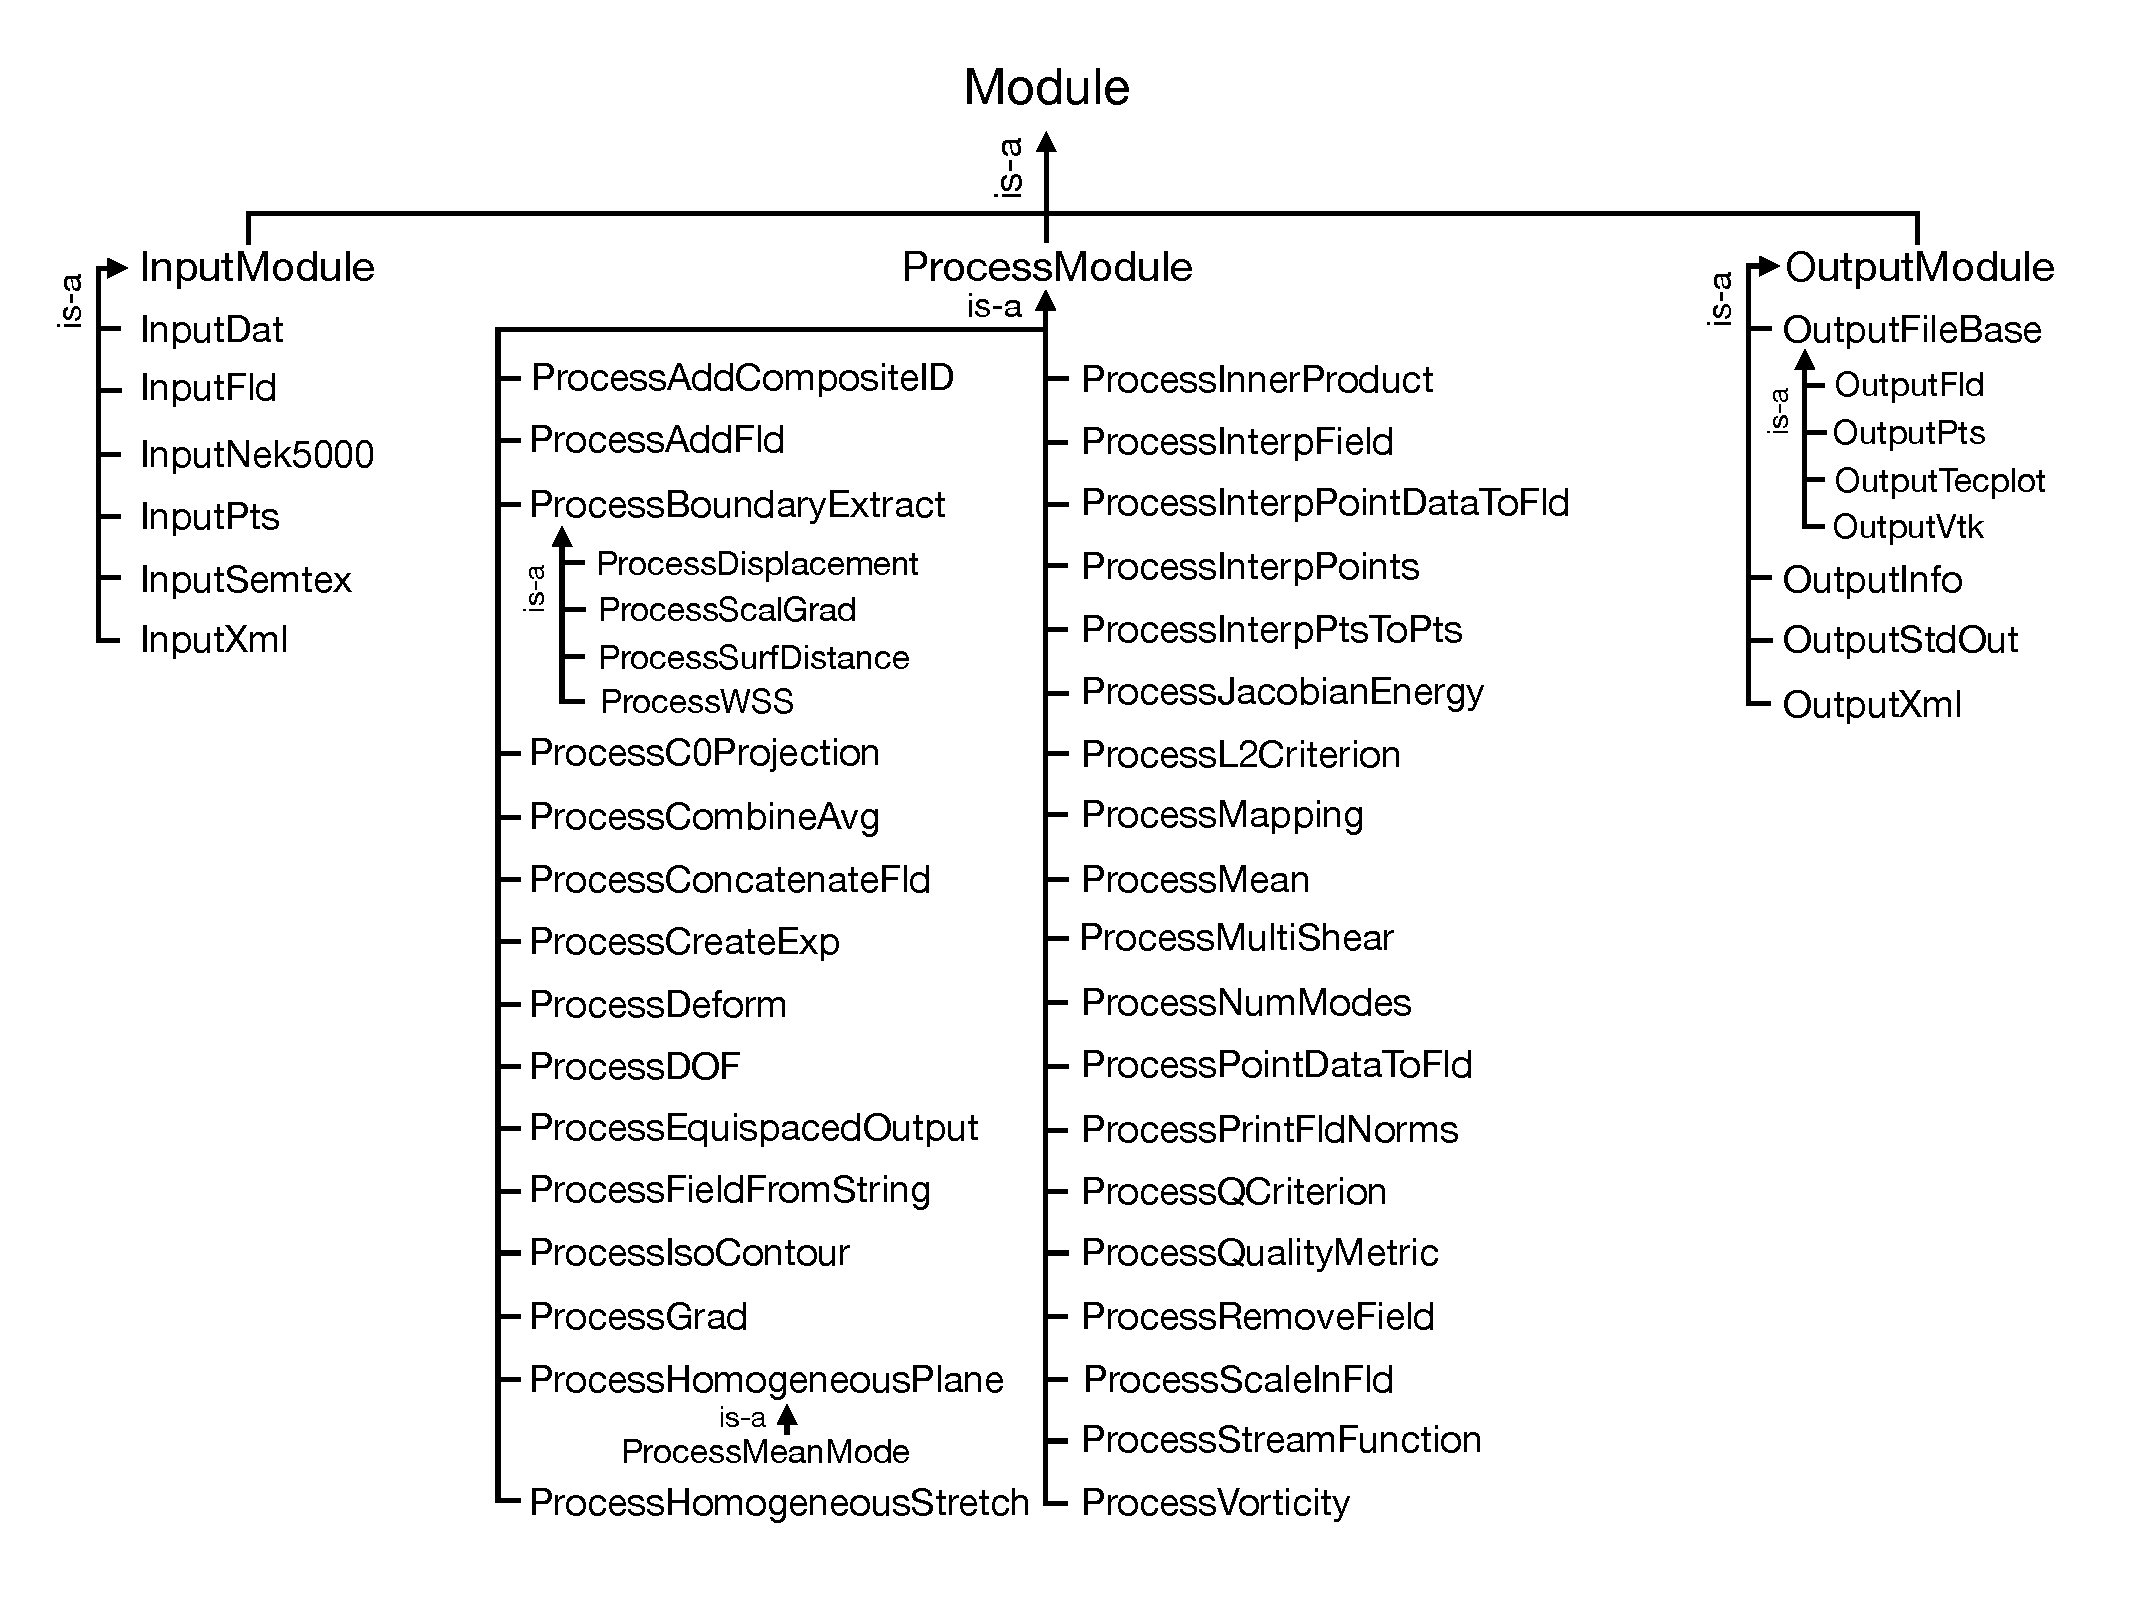
\includegraphics[width=\linewidth]{library/FieldUtils/img/ModuleInheritance.pdf}
\label{fig:module_inheritance}
\caption{\texttt{Module} class inheritance} 
\end{figure}